\subsubsection{エラー率が内部栄養濃度$y$に依存する場合}
次に,エラー率が細胞内の栄養濃度$y$に依存して
\begin{equation}
  \epsilon = \frac{\delta}{K + y} \label{erry}
\end{equation}
と書ける場合を考える.
この場合に,$K=1$として同様の数値計算を行い,$\delta$と定常成長速度$\mu$の関係をプロットした(図\ref{fig:n_vs_mu_K1s1}).
次に,この図を参考に,成長に必要な外部栄養濃度$n^*$をこれまでとまったく同じように定義した.
そして,$K=1,10,100$のそれぞれについて,$\delta/K$と$n^*$の関係をプロットした(図\ref{fig:err_vs_n_errslope_s1}).
この図からも,図\ref{fig:err_vs_n_errslope_s0}と同じく,$\delta/K$が大きくなると理論線(式\eqref{nast_errconst}で$\epsilon=\delta/K$としたもの)から外れることと,$K$が大きいとプロットが理論線から外れ始める$\delta/K$の値が大きくなることが読み取れる.
それらについての考察は同様なので省略する.

一方で,図\ref{fig:err_vs_n_errslope_s0}と図\ref{fig:err_vs_n_errslope_s1}を比べると,同じ$K$の値に対し,エラー率が$x$に依存しているときに比べて,$y$に依存しているときの方が$n^*$が小さく済むことが読み取れる.
これについては,以下のように説明ができる.
まず,成長できる最小限近くの外部栄養濃度$n\approx n^*$において,$\mu$が小さいことから$x$は小さい.
その一方で,$y$は拡散流入により$n^*$近くの値になる.
つまり,$x$より$y$の方が大きいため,エラー率は式\eqref{errx}よりも式\eqref{erry}の方が小さくなる.
その結果,エラー率が$y$に依存する場合の方が$n^*$が少なく済むと考えられる.

\begin{figure}[htbp]
  \centering
  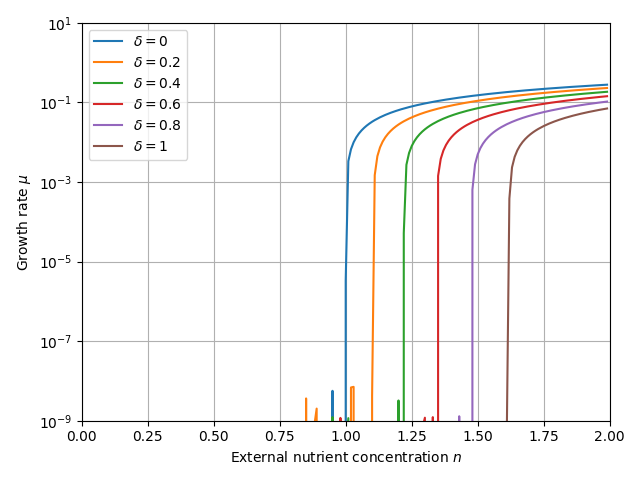
\includegraphics[width=10cm]{n_vs_mu_K1s1_errslope.png}
  \caption{エラー率が$y$に式\eqref{erry}の形($K=1$,$\delta=0,0.2,0.4,0.6,0.8,1$)で依存するとして計算した,時刻$t=10^5$における外部栄養濃度$n$と成長速度$\mu$の関係(刻み幅,初期濃度,パラメータの取り方は図\ref{fig:n_vs_mu_errconst}のときと同様である.).この場合,エラー率が$x$依存する場合と比べて,成長に必要な$n$は少なく済む.}
  \label{fig:n_vs_mu_K1s1}
\end{figure}

\begin{figure}[htbp]
  \centering
  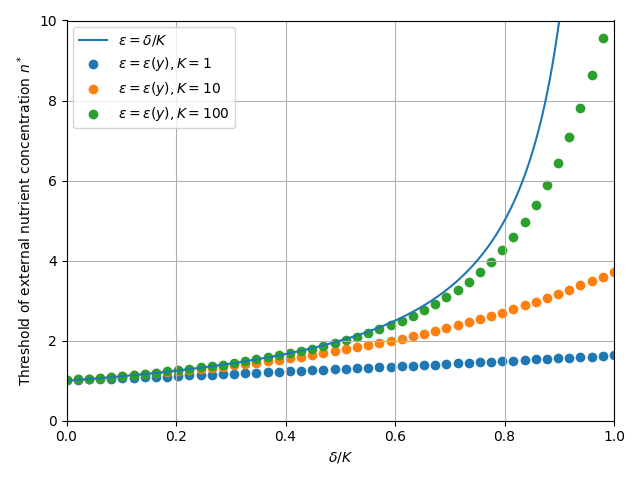
\includegraphics[width=10cm]{err_vs_n_errslope_s1_K.png}
  \caption{エラー率が$y$に式\eqref{erry}の形($K=1,10,100$)で依存するとして計算した,$\delta$と成長に必要な($\mu > 10^{-3}$となる最小の)外部栄養濃度$n^*$の関係($n$は刻み幅0.01で変更した.それ以外のパラメータは図\ref{fig:n_vs_mu_errconst}と同様である.).}
  \label{fig:err_vs_n_errslope_s1}
\end{figure}
